\documentclass[11pt,spanish]{article}

\usepackage{listings}             
\usepackage{anysize} 
\usepackage{graphicx}
\usepackage[spanish]{babel}
\usepackage[utf8]{inputenc}
\usepackage{xcolor}
\usepackage{wrapfig}


\lstset{language=Python}
\marginsize{1cm}{1cm}{2cm}{2cm}
\selectlanguage{spanish}
\lstset{
language=Python,
 backgroundcolor=\color{red!75!green!50!blue!25},
 frame=single,
literate=
  {á}{{\'a}}1 {é}{{\'e}}1 {í}{{\'i}}1 {ó}{{\'o}}1 {ú}{{\'u}}1
  {Á}{{\'A}}1 {É}{{\'E}}1 {Í}{{\'I}}1 {Ó}{{\'O}}1 {Ú}{{\'U}}1
  {à}{{\`a}}1 {è}{{\`e}}1 {ì}{{\`i}}1 {ò}{{\`o}}1 {ù}{{\`u}}1
  {À}{{\`A}}1 {È}{{\'E}}1 {Ì}{{\`I}}1 {Ò}{{\`O}}1 {Ù}{{\`U}}1
  {ä}{{\"a}}1 {ë}{{\"e}}1 {ï}{{\"i}}1 {ö}{{\"o}}1 {ü}{{\"u}}1
  {Ä}{{\"A}}1 {Ë}{{\"E}}1 {Ï}{{\"I}}1 {Ö}{{\"O}}1 {Ü}{{\"U}}1
  {â}{{\^a}}1 {ê}{{\^e}}1 {î}{{\^i}}1 {ô}{{\^o}}1 {û}{{\^u}}1
  {Â}{{\^A}}1 {Ê}{{\^E}}1 {Î}{{\^I}}1 {Ô}{{\^O}}1 {Û}{{\^U}}1
  {œ}{{\oe}}1 {Œ}{{\OE}}1 {æ}{{\ae}}1 {Æ}{{\AE}}1 {ß}{{\ss}}1
  {ű}{{\H{u}}}1 {Ű}{{\H{U}}}1 {ő}{{\H{o}}}1 {Ő}{{\H{O}}}1
  {ç}{{\c c}}1 {Ç}{{\c C}}1 {ø}{{\o}}1 {å}{{\r a}}1 {Å}{{\r A}}1
  {€}{{\EUR}}1 {£}{{\pounds}}1
}


\title{\vspace{-3cm}\begin{flushleft}\textbf{Actividad 5}\end{flushleft}}
\author{\hspace{-9.6cm}\textsc{Andrés Ignacio Rodríguez Mendoza}}
\date{}

\begin{document}

\begin{wrapfigure}{r}{0.2\textwidth}
  \begin{center}
   \vspace{-5.4cm} 
\includegraphics[width=0.15\textwidth]{uni}
  \end{center}
\end{wrapfigure}

\maketitle  
\begin{center}
\rule{\textwidth}{1pt}
\end{center}

\section*{Introducción}
El ``péndulo simple'' es una idealización de un ``péndulo real'' en un sistema aislado usando los siguientes supuestos:se considera una cuerda sin masa, inextensible y siempre tensa, el objeto es una masa puntual, el movimiento ocurre en dos dimensiones, se desprecia fricción o resistencia al aire, el campo gravitacional es uniforme, y el soporte está fijo.\\ \\
La ecuación diferencial que representa el movimiento de un péndulo simple es
\begin{equation}
\frac{d^2\theta}{dt^2} + \frac{g}{l} \sin \theta = 0
\end{equation}
donde g es la aceleración debido a la gravedad, $l$ es la longitud de la cuerda, y $\theta$ es el desplazamiento angular.\\ \\
En este proyecto se resuelve numericamente la ecuación del péndulo. La herramienta \textit{scipy.integrate.odeint} de \textit{SciPy} integra un sistema de ecuaciones diferenciales usando \textit{lsoda} de la librería \textit{Odepack} de Fortran. Se grafican los resultados utilizando la librería \textit{matplotlib.pyplot}, una colección de funciones con estilo de comando que hace a \textit{matplot} trabajar como Matlab.
\section*{Código}

\begin{lstlisting} % Start your code-block}

from scipy.integrate import odeint
import matplotlib.pyplot as plt

def pend(y, t, b, c):
    theta, omega = y
    dydt = [omega, -(b/c)*np.sin(theta)]
    return dydt

g = 9.81


l1=5
l2=10

y0 = [np.pi - 0.1, 0.0]

t = np.linspace(0, 50, 101)


sol1 = odeint(pend, y0, t, args=(g,l1))

plt.subplot(211)
plt.plot(t, sol1[:, 0], 'b', label='theta(t)')
plt.grid()
plt.ylabel('theta')

plt.title('Longitud de péndulo l = 5 m')

plt.subplot(212)
plt.plot(t, sol1[:, 1], 'g', label='omega(t)')
plt.grid()
plt.ylabel('omega')
plt.xlabel('t')


plt.show()

sol2 = odeint(pend, y0, t, args=(g,l2))

plt.subplot(211)
plt.plot(t, sol2[:, 0], 'b', label='theta(t)')
plt.grid()
plt.ylabel('theta')

plt.title('Longitud de péndulo l = 10 m')

plt.subplot(212)
plt.plot(t, sol2[:, 1], 'g', label='omega(t)')
plt.grid()
plt.ylabel('omega')
plt.xlabel('t')


plt.show()
\end{lstlisting}

\section*{Gáficas}

\centering

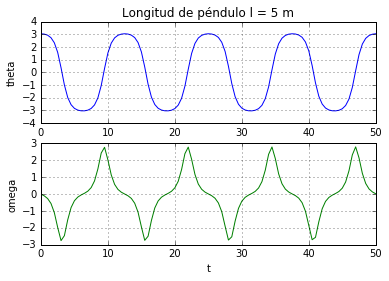
\includegraphics{graph1}\\
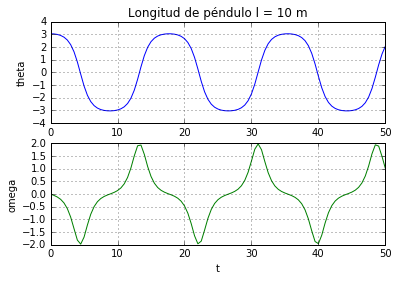
\includegraphics{graph2}\\





\end{document}

